\chapter{Eksperyment}

W końcowym etapie pracy postanowiono przeprowadzi\'c analizę jakościową zaimplementowanego
systemu. W tym celu posłużono się i obliczono wartości dwóch najpopularniejszych współczynników
używanych do oceny poprawności działania systemów biometrycznych:

\begin{itemize}
  \item FAR \textit{(ang. False Acceptance Rate)} - miara prawdopodobieństwa nieprawidłowego zaakceptowania
  obrazu
  \item FRR \textit{(ang. False Rejection Rate)} - miara prawdopodobieństwa nieprawidłowego odrzucenia
  obrazu
\end{itemize}

W dalszej części tego rozdziału zawarty został opis eksperymentu oraz zasobów użytych do jego
przeprowadzenia.

\section{Wykorzystane wska\'zniki}

Tak jak wspomniano we wstępie niniejszego rozdziału, do określenia dokładności działania zaimplementowanego
systemu użyte zostały wska\'zniki FAR oraz FRR. \newline

FAR \textit{(ang. False Acceptance Rate)} definiuje prawdopodobieństwo zaistnienia sytuacji, w której
osoba nieautoryzowana może zosta\'c nieprawidłowo rozpoznana przez system biometryczny. Zwykle wska\'znik ten
jest uważany za najważniejszy, ze względu na bezpośrednie opisywanie prawdopodobieństwa narusznia
bezpieczeństwa systemu. Wska\'znik ten można zdefiniowa\'c w następujący sposób:

\begin{equation}
  \mathit{FAR} = \frac{N_{\mathit{fa}}}{N_{t}},
\end{equation}

\noindent
gdzie:\\
\indent $\mathit{FAR}$ - False Acceptance Rate,\\
\indent $N_{\mathit{fa}}$ - liczba nieprawidłowo zaakceptowanych dopasowań,\\
\indent $N_{t}$ - liczba wszystkich prób dopasowań.\newline

Drugim wska\'znikiem wykorzystywanym do określenia jakości działania systemu jest FRR \textit{(ang. False Rejection Rate)}.
Mówi on o prawdopodobieństwu nieprawidłowego odrzucenia osoby identyfikowanej. Jest to wska\'znik, który
nie wskazuje wad w bezpieczeństwie działania systemu, natomiast może definiowa\'c to jak
szybko będzie dany system działał oraz ilukrotnie potencjalny użytkownik będzie musiał powtórzy\'c
proces autoryzacji. Wska\'znik ten można zdefiniowa\'c w sposób opisany przez poniższe równianie:

\begin{equation}
  \mathit{FRR} = \frac{N_{\mathit{fr}}}{N_{t}},
\end{equation}

\noindent
gdzie:\\
\indent $\mathit{FRR}$ - False Rejection Rate,\\
\indent $N_{\mathit{fr}}$ - liczba nieprawidłowo odrzuconych dopasowań,\\
\indent $N_{t}$ - liczba wszystkich prób dopasowań.\newline

Za najlepsze rozwiązanie systemu biometrycznego można uzna\'c takie, które jednocześnie zapewnia
najmniejszą wartoś\'c obu tych współczynników (z naciskiem na FAR). Takie podejście pozwala zachowa\'c balans między bezpieczeństwem
systemu, a jego użyteczńością.

\begin{figure}[ht]
  \centering
  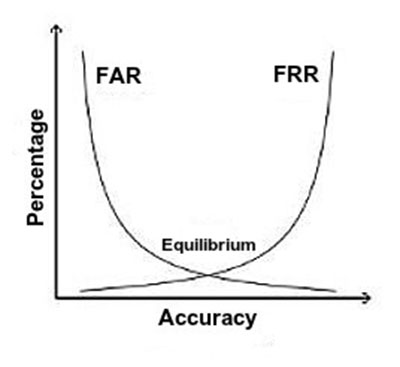
\includegraphics[width=0.7\textwidth]{images/experiment/frrfardiagram.jpg}
  \caption{Balans między współczynnikami FAR oraz FRR.}
\end{figure}

\section{Opis eksperymentu}

W celu określenia jakości działania zaimplementowanego systemu postanowiono obliczy\'c wartości powyżej opisanych wska\'zników
przy użyciu różnych wartości parametrów metod poszczególnych etapów przetwarzania. We wszystkich przypadkach zdecydowano
się na użycie metody segmentacji zaproponowanej przez Daugmana \cite{DaugmanHowIrisRecognitionWorks}, która na podstawie obserwacji
określona została jako najlepiej działająca z tych dostępnych w aplikacji. Zastosowana została ona w dwóch wariantach:
bez wykrywania powiek oraz wykrywaniem powiem przy użyciu aproksymacji parabolą. Jako podstawowe wartości parametrów
metod wykorzystano te zaproponowane w swojej pracy przez Maseka \cite{masek}, który opisał je jako optymalne. Pozostałe
przypadki w eksperymencie pokazują odchylenia od tych wartości. Poniżej przedstawiono zestawienie parametrów podstawowych:

\begin{itemize}
  \item normalizacja - rozdzielczoś\'c kątowa równa 260, rozdzielczoś\'c promieniowa równa 32 (odpowiednio szerokoś\'c i wysokoś\'c obrazu)
  \item kodowanie - częstotliwoś\'c środkowa filtru równa 18 pikseli, przepustowoś\'c $\sigma/f$ wynosząca 0.5,
  \item dopasowanie - próg odległości Hamminga równy 0.35, iloś\'c przesunię\'c wynosząca 8.
\end{itemize}

Do przeprowadzenia eksperymentu wykorzystana została baza danych zdję\'c oczu CASIA w wersji pierwszej [zasób: \ref{web:CASIA}].
Składa się ona z 756 obrazów przedstawiających 108 unikalnych tęczówek. Zdjęcia robione były obu oczom w dwóch
sesjach. W ramach sesji pierwszej pobieranie były trzy, a w ramach drugiej sesji cztery zdjęcia. Wszystkie z nich
są w formacie \textit{BMP} i mają rozdzielczoś\'c 320x280 pikseli. Na rysunku poniżej (rysunek \ref{fig:casiaExample})
przedstawione zostały przykładowe obrazy z tej bazy:\newline

\begin{figure}[h]
  \centering
  \begin{subfigure}[b]{\textwidth}
    \centering
    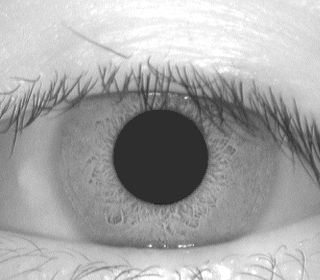
\includegraphics[width=0.45\textwidth]{images/experiment/CasiaExampleOneLeft.png}
    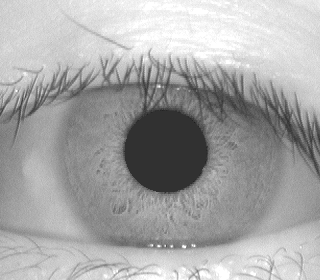
\includegraphics[width=0.45\textwidth]{images/experiment/CasiaExampleOneRight.png}
  \end{subfigure}
  \begin{subfigure}[b]{\textwidth}
    \centering
    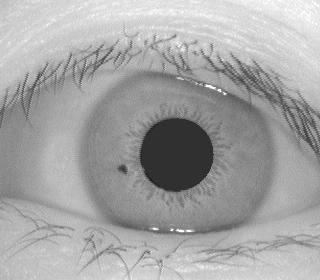
\includegraphics[width=0.45\textwidth]{images/experiment/CasiaExampleTwoLeft.png}
    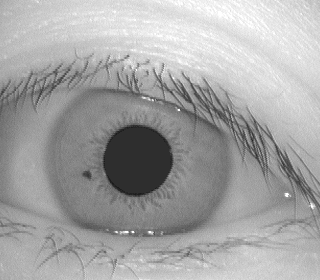
\includegraphics[width=0.45\textwidth]{images/experiment/CasiaExampleTwoRight.png}
  \end{subfigure}
  \caption{Przykładowe zdjęcia z bazy danych CASIA. Z lewej strony
  znajduje się obraz pobrany w pierwszej sejsi, a zdrugiej strony obraz pobrany w drugiej sesji.}
  \label{fig:casiaExample}
\end{figure}

Ze względu na problemy występujące podczas procesu segmentacji, eksperyment przeprowadzony został dla pierwszych
300 obrazów znajdujących się w bazie danych odpowiadających 47 unikalnym tęczówkom. W trakcie eksperymentu
pojawiły się także inne problemy związane z wyznaczaniem powiek, które skutkowały wyznaczeniem maski zakłóceń
obejmującej cały obszar zdjęcia. W takich wypadkach obrazy nie były poddawane eksperymentowi, a liczba pominiętych
obrazów uwzględniona została w trakcie obliczania współczynników FAR oraz FRR.

\section{Wyniki eksperymentu}



\rowcolors{2}{gray!10}{white}
\begin{table}[ht]
  \centering
  \begin{tabular}{c|c|c|c}
    \rowcolor{gray!20}
    Metoda segmentacji & Metoda wykrywania powiek & FAR & FRR \\
    \hline\hline
    Daugman & Brak & 0.0000 & 0.0094 \\
    \hline
    Daugman & Aproksymacja parabolą & 0.0001 & 0.0076 \\
  \end{tabular}
  \caption{Porównanie współczynników FAR i FRR dla różnych metod wykrywania powiek.}
\end{table}

Wszystkie dalsze sa segmentacja metoda daugmana.

Brak wykrywania powiek:

\rowcolors{2}{gray!10}{white}
\begin{table}[ht]
  \centering
  \begin{tabular}{c|c|c}
    \rowcolor{gray!20}
    Próg odległości Hamminga & FAR & FRR \\
    \hline\hline
    0.25 & 0.0000 & 0.0198 \\
    \hline
    0.35 & 0.0000 & 0.0094 \\
    \hline
    0.45 & 0.0282 & 0.0004 \\
    \hline
    0.5 & 0.9698 & 0.0000 \\
  \end{tabular}
  \caption{Porównanie współczynników FAR i FRR dla różnych wartości progowych odległości Hamminga
  przy braku wykrywania powiek.}
\end{table}

Aproksymacja parabola:

\rowcolors{2}{gray!10}{white}
\begin{table}[ht]
  \centering
  \begin{tabular}{c|c|c}
    \rowcolor{gray!20}
    Próg odległości Hamminga & FAR & FRR \\
    \hline\hline
    0.25 & 0.0000 & 0.0196 \\
    \hline
    0.35 & 0.0002 & 0.0077 \\
    \hline
    0.45 & 0.0387 & 0.0003 \\
    \hline
    0.5 & 0.9702 & 0.0000 \\
  \end{tabular}
  \caption{Porównanie współczynników FAR i FRR dla różnych wartości progowych odległości Hamminga
  z wykorzystaniem aproksymacji parabolicznej do wykrywania powiek.}
\end{table}

Przesuniecia - dla aproksymacji parabola

Brak wykrywania powiek:

\rowcolors{2}{gray!10}{white}
\begin{table}[ht]
  \centering
  \begin{tabular}{c|c|c}
    \rowcolor{gray!20}
    Liczba przesunię\'c & FAR & FRR \\
    \hline\hline
    3 & 0.0003 & 0.0098 \\
    \hline
    8 & 0.0000 & 0.0094 \\
  \end{tabular}
  \caption{Porównanie współczynników FAR i FRR dla różej ilości przesunię\'c wzoru tęczówki w procesie dopasowania
  przy braku wykrywania powiek.}
\end{table}

Aproksymacja parabola:

\rowcolors{2}{gray!10}{white}
\begin{table}[ht]
  \centering
  \begin{tabular}{c|c|c}
    \rowcolor{gray!20}
    Liczba przesunię\'c & FAR & FRR \\
    \hline\hline
    3 & 0.0001 & 0.0082 \\
    \hline
    8 & 0.0002 & 0.0077 \\
  \end{tabular}
  \caption{Porównanie współczynników FAR i FRR dla różej ilości przesunię\'c wzoru tęczówki w procesie dopasowania
  z wykorzystaniem aproksymacji parabolicznej do wykrywania powiek.}
\end{table}

Rozmiar obrazu znormalizowanego:

Brak wykrywania powiek:

\rowcolors{2}{gray!10}{white}
\begin{table}[ht]
  \centering
  \begin{tabular}{c|c|c|c}
    \rowcolor{gray!20}
    Rozdzielczoś\'c kątowa & Rozdzielczoś\'c promieniowa & FAR & FRR \\
    \hline\hline
    120 & 16 & 0.0027 & 0.0073 \\
    \hline
    240 & 32 & 0.0000 & 0.0094 \\
    \hline
    360 & 64 & 0.0000 & 0.0109 \\
  \end{tabular}
  \caption{Porównanie współczynników FAR i FRR dla różnych rozmiarów obrazu znormalizowanego
  przy braku wykrywania powiek.}
\end{table}

Aproksymacja parabolą:

\rowcolors{2}{gray!10}{white}
\begin{table}[ht]
  \centering
  \begin{tabular}{c|c|c|c}
    \rowcolor{gray!20}
    Rozdzielczoś\'c kątowa & Rozdzielczoś\'c promieniowa & FAR & FRR \\
    \hline\hline
    120 & 16 & 0.0035 & 0.0065 \\
    \hline
    240 & 32 & 0.0002 & 0.0077 \\
    \hline
    360 & 64 & 0.0001 & 0.0091 \\
  \end{tabular}
  \caption{Porównanie współczynników FAR i FRR dla różnych rozmiarów obrazu znormalizowanego
  z wykorzystaniem aproksymacji parabolicznej do wykrywania powiek.}
\end{table}

Wartoś\'c parametru $\sigma/f$

Brak wykrywania powiek:

\rowcolors{2}{gray!10}{white}
\begin{table}[ht]
  \centering
  \begin{tabular}{c|c|c}
    \rowcolor{gray!20}
    $\sigma/f$ & FAR & FRR \\
    \hline\hline
    0.3 & 0.0003 & 0.0080 \\
    \hline
    0.5 & 0.0000 & 0.0094 \\
    \hline
    0.75 & 0.0000 & 0.0100 \\
  \end{tabular}
  \caption{Porównanie współczynników FAR i FRR dla różnych wartości parametru $\sigma/f$ filtru Gabora
  przy braku wykrywania powiek.}
\end{table}


Aproksymacja parabola:

\rowcolors{2}{gray!10}{white}
\begin{table}[ht]
  \centering
  \begin{tabular}{c|c|c}
    \rowcolor{gray!20}
    $\sigma/f$ & FAR & FRR \\
    \hline\hline
    0.3 & 0.0009 & 0.0069 \\
    \hline
    0.5 & 0.0002 & 0.0077 \\
    \hline
    0.75 & 0.0008 & 0.0084 \\
  \end{tabular}
  \caption{Porównanie współczynników FAR i FRR dla różnych wartości parametru $\sigma/f$ filtru Gabora
  z wykorzystaniem aproksymacji parabolicznej do wykrywania powiek.}
\end{table}
